\parindent=0em
\subsection{Aplicaciones de pruebas}
\noindent

Debido al extenso número de factores a considerar a la hora de realizar las pruebas, han sido implementadas dos aplicaciones para automatizarlas y extraer los datos de ellas.\\

El resultado obtenido no se limita a una única ejecución de la prueba para evitar producir sesgo en los datos. Cada prueba es realizada desde distintas perspectivas (mínimo 2) y así poder considerar varios factores. Estos pueden ser, por ejemplo, la luz natural del entorno o los objetos que en este se encuentren.\\ 

\begin{itemize}
    \item \textbf{Aplicación ARCore}: Esta aplicación realiza todas las comprobaciones necesarias para valorar el estado de la oclusión de un conjunto de elementos determinados así como del rendimiento los mismos.\\
    
    El uso ideal se conseguiría mediante un archivo de vídeo sobre el que se iterarían todas las pruebas. Sin embargo ARCore no utiliza únicamente los datos extraídos de la entrada de vídeo para calcular la profundidad del entorno. A estos datos les añade los obtenidos de los distintos sensores como pueden ser el giróscopo o el acelerómetros, para medir rotaciones y posiciones respectivamente.\\
    
    La aplicación cuenta con un \textit{Asset} para facilitar la medición de los datos llamado Graphy ~\cite{Graphy}. Este proporciona los \textit{Frames por segundo (FPS)} de la aplicación, el uso de la memoria y el consumo de la CPU, así como todas las características internas del dispositivo.\\
    
    En la interfaz se pueden encontrar todas las opciones necesarias para generar las pruebas (referencias a la (figura \ref{fig:Trigonometry})): 
    \begin{itemize}
         \item \textbf{1. Start Point Cloud}: Sirve para generar la nube de puntos de manera que esta se pueda ver desde la aplicación.
         \item \textbf{2. Test Visualization}: Siempre y cuando la nube de puntos esté activada, esta opción ejecuta la batería de pruebas para comprobar la oclusión.
         \item \textbf{3. Start Time Test}: Activa y desactiva la prueba para comprobar el tiempo de generación de la nube de puntos.
         \item \textbf{4. Chg. Max. Ptos}: Cambia el número de puntos máximos que puede tener la nube de puntos.
         \item \textbf{5. Chg. Ptos. \textit{Frame}}: Modifica el número de puntos en la nube máximo que se pueden generar por \textit{frame}.
         \item \textbf{6. Chg. Forma}: Intercambia las distintas formas para probar las variantes de la oclusión.
         \item \textbf{7. Capturar pantalla}: Siempre que la nube de puntos esté activada, genera una captura del estado de la pantalla.
         \item \textbf{8. Medidor de pruebas}: Utilizado para visualizar todos los estados de las interacciones anteriores.
         \item \textbf{9. Datos Graphy}: Datos de \textit{Graphy} como el rendimiento en \textit{FPS} o la memoria utilizada.
       
    \begin{figure}[h]
    \centering
    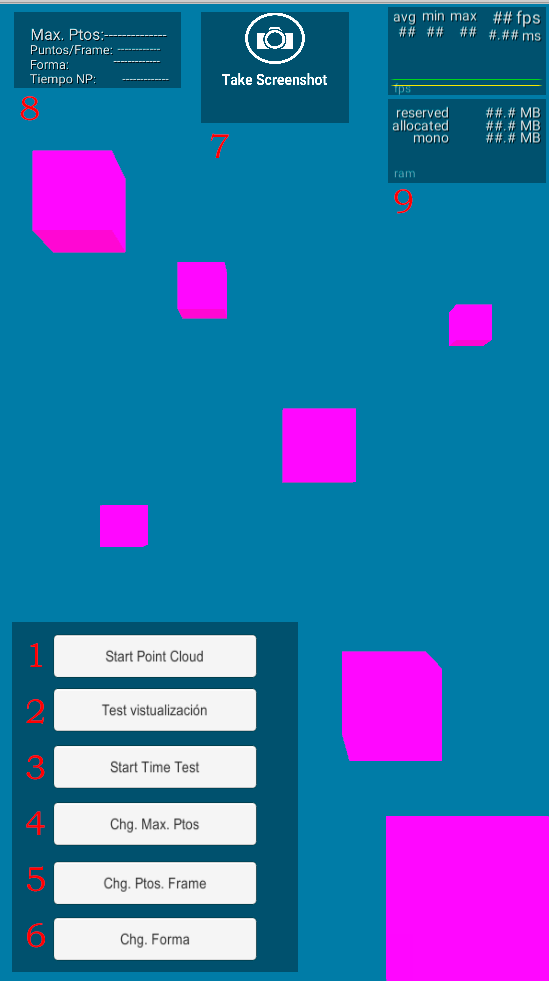
\includegraphics[scale=0.35]{Images/NubeDePuntos/UnityApp.png}
    \caption[Vista principal de la aplicación para la generación de pruebas.]{Vista principal de la aplicación para la generación de pruebas.}
    \label{fig:AppUnity}
    \end{figure}
     \end{itemize}
     \item   \textbf{Test Visualization}: Debido a que esta prueba engloba todos los apartados dentro de la aplicación anterior, se detallará en más profundidad su uso.\\
        
    Para el uso de este test se ha de activar la nube de puntos, por lo que se pulsará el botón \textit{1. Start Point Cloud}.\\ 
        
    Una vez esté completa la nube de puntos deseada para generar la oclusión, habrá que pulsar el botón \textit{2. Test Visualization} para comenzar la prueba. Cabe destacar en este punto que para el correcto funcionamiento de la siguiente aplicación, el dispositivo ha de encontrarse totalmente estático. Este proceso se explicará más en detalle en el apartado \textit{Errores de las pruebas}.\\
    
    Una vez pulsado este botón, la aplicación ejecutará el script C\# que controla toda la prueba. Este realizará la siguiente serie de acciones:
        
         \begin{itemize}
            \item \textbf{Obtención de la nube de puntos}: Gracias al script PointCloudEditor, es posible acceder a la nube de puntos en cualquier momento o estado. Esta se guardará en una lista de \textit{Vector3}, ya que la nube de puntos únicamente son posiciones en el espacio, y desactivará la nube para que no interfiera más en las pruebas.
         
            \item \textbf{Ocultación del HUD}: Para que las pruebas se realicen con la máxima fiabilidad posible, se procede a ocultar todo el HUD de la aplicación.
            Todo el proceso descrito a continuación se engloba dentro de una corrutina para facilitar la visualización de errores durante ejecución y para poder realizar las capturas con la cámara.
          
            \item \textbf{Creación de los puntos}: En cada una de las posiciones de la nube de puntos se generará un objeto mediante la función \textit{Instantiate} de Unity, y este se almacenará dentro de una lista de ``GameObjects'' para poder utilizarlos en el futuro.
            
            \item \textbf{Bucle principal}: Dentro de este apartado, se realizará la comprobación por cada forma y por cada tamaño. Por defecto, la aplicación cuenta con cinco formas distintas (Esfera, cubo, quad, cilindro y cápsula) y con cinco tamaños distintos (desde 0,01 hasta 0,05). Existen varios bucles anidados que recorren todas estas posibilidades. En primer lugar, un bucle recorre todas las formas y a cada uno de los puntos anteriormente creados, les aplica la forma que le corresponda. En segundo lugar, dentro de ese mismo bucle, existe otro que recorre todos los tamaños posibles y aplica a cada objeto el tamaño que en este caso tenga que comprobar.
             
            \item \textbf{Captura}: Una vez se tenga un tamaño concreto para todas las posiciones de la nube de puntos, mediante la opción disponible dentro de las corrutinas de unity \textit{``yield return new WaitForEndOfFrame()''} esperará a que el \textit{frame} termine para poder realizar la captura de pantalla. Esto se debe a que al estar dentro de una hebra separada del bucle principal de Unity, la captura de pantalla se puede realizar sin que se haya pintado el \textit{frame} anterior, por lo que nos aseguramos que el paso de \textit{renderizado} de Unity ya se haya realizado. Acto seguido, realizamos la captura y volvemos a realizar el mismo paso de esperar al final del \textit{frame} para asegurar que se ha realizado correctamente.
            
            \item \textbf{Imágenes vacías}: Finalmente, se crearán dos imágenes particulares. Una de ellas, es una imagen sin ningún tipo de elemento virtual, únicamente con la imagen de la cámara. La otra consiste en un fondo negro únicamente con los elementos virtuales. Estas dos imágenes en el futuro servirán para crear la que llamaremos imagen ``Desired'', que representará el estado óptimo esperado por la oclusión.
    
    \end{itemize}
    
    \item \textbf{Aplicación de comparación de imágenes}: En este caso la aplicación realiza toda la comprobación de imágenes necesaria para la prueba \textit{Test Visualization} de la aplicación anterior. Consiste en un script escrito en Python.\\
    
    Esta busca dentro de un directorio dado todas las carpetas que este contenga. En nuestro ejemplo, ya que se realizaron 5 pruebas, se generaron 5 carpetas llamadas \textit{VistaN}, donde N es el numero de la prueba. Acto seguido, buscará una subcarpeta llamada \textit{Images}, donde se encuentran todas las imágenes generadas por la aplicación de Unity.\\
    
    En el mismo directorio \textit{VistaN}, también encontramos la imagen \textit{Desired} antes mencionada así como las dos originales que dan forma a esta. Una vez encontradas todas las imágenes, se comparan una a una con \textit{Desired}, generando en una nueva carpeta llamada \textit{Structural Similarity} una imagen por cada imagen tomada, del resultado de comparación entre \textit{Desired} y las originales. Esto sólo nos servirá como referencia para validar que dicha comparación es correcta.\\
    
    A su vez, en el directorio raíz donde se ejecuta la aplicación también se generan una serie de archivos CSV, uno por cada carpeta \textit{VistaN}, llamado \textit{ResultsVistaN}. En ellos encontramos todos los datos de cada una de las pruebas. La forma del objeto, su tamaño y el porcentaje de acierto que ha obtenidos. Para finalizar, se genera un último archivo CSV, llamado \textit{Final\_Results}. En este encontramos la media de todas y cada una de las pruebas unidas. Es decir, la media del resultado de cada una de las formas y tamaños para todas las pruebas \textit{VistaN}. 
    
    \begin{figure}[H]
    \centering
    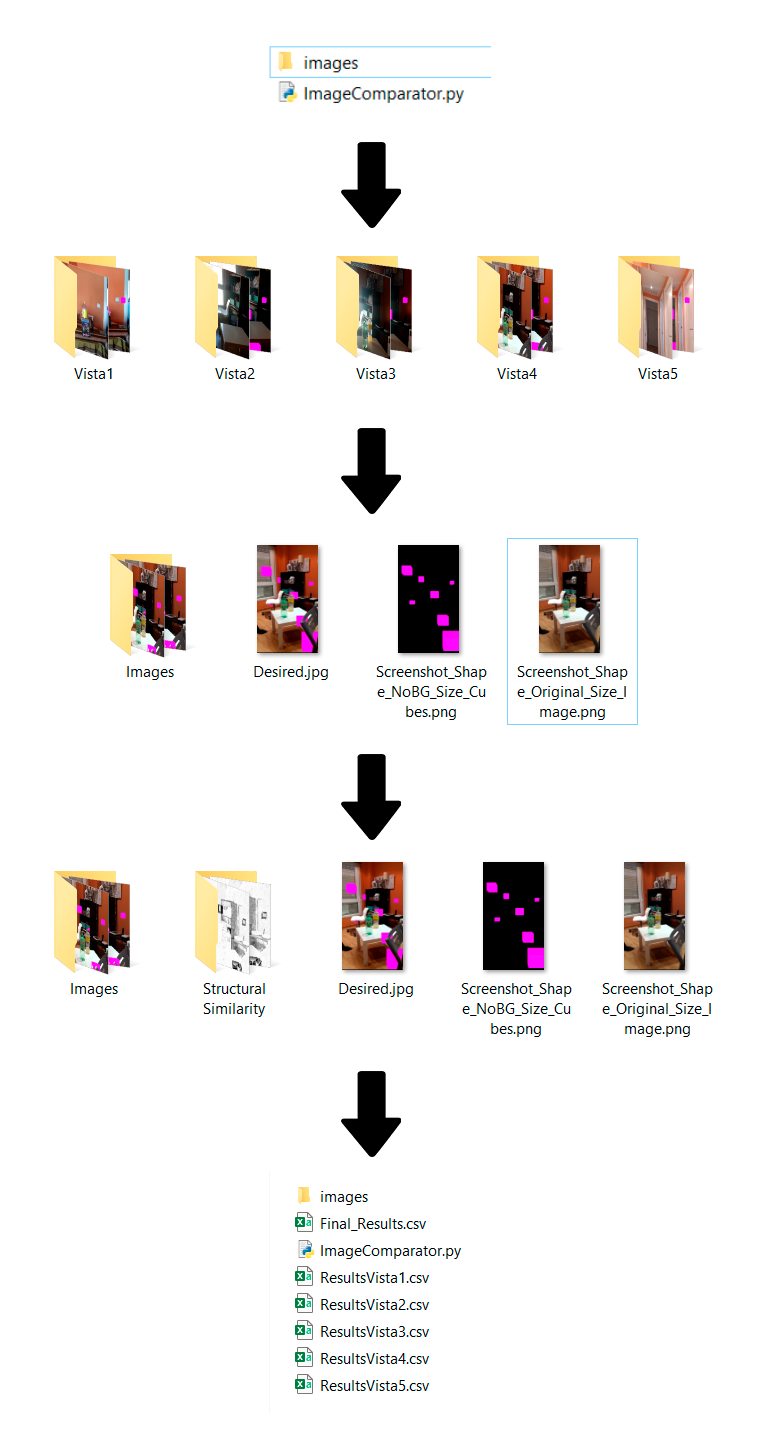
\includegraphics[scale=0.20]{Images/NubeDePuntos/CarpetasPruebas.png}
    \caption[Estructura de las carpetas para comparar imágenes.]{Estructura de las carpetas para comparar imágenes.}
    \label{fig:CarpetasPruebas}
    \end{figure} 
    
\end{itemize}


